% !TEX root = ./Report_homework1_final.tex
\documentclass[a4paper,11pt]{article}
\usepackage[utf8]{inputenc}
\usepackage{graphicx}
\usepackage{hyperref}
\usepackage{amsmath}
\usepackage{amsfonts} 
\usepackage{booktabs}
\usepackage{caption}
\usepackage{float}

% Dati studente
\title{\textbf{Homework 1: Robot Control}}
\author{Sara Cristina Basco (Student Number: 2256687)}
\date{\today}

\begin{document}

\maketitle

\section{Introduction}
The objective of this project is to learn a control function for a robotic arm without prior knowledge of its kinematic model. Specifically, the task consists in approximate the function $dq = f(x, q, dx)$, which predicts the necessary joint displacements given the current end-effector position, current joint configuration, and the desired end-effector displacement.

This problem is framed as a supervised regression task. The proposed approach is evaluated on all robotic agents provided in the dataset.

\section{Experimental Setup}
This work evaluates the learning methodology on three variations of the “Reacher" robotic arm, spanning from a simple planar manipulator to a redundant spatial robot.

\subsection{Robots Description}
All robotic agents are simulated using the ROS~2 framework. Three configurations with increasing levels of complexity are considered:

\begin{itemize}
    \item \textbf{Reacher3 (Planar):} A 3-DOF (Degrees of Freedom) arm operating in a 2D plane. The end-effector position is defined by $(x, y)$ coordinates. Since the task space is 2D and the joint space is 3D, the robot has 1 degree of redundancy.
    \item \textbf{Reacher4 (Spatial):} A 4-DOF arm operating in 3D space. The end-effector position involves $(x, y, z)$ coordinates. With 4 joints controlling 3 spatial coordinates, this robot is redundant.
    \item \textbf{Reacher6 (Spatial):} A 6-DOF arm operating in 3D space. This is a highly redundant manipulator, allowing for complex poses to reach the same target position.
\end{itemize}

\begin{figure}[h!]
    \centering
    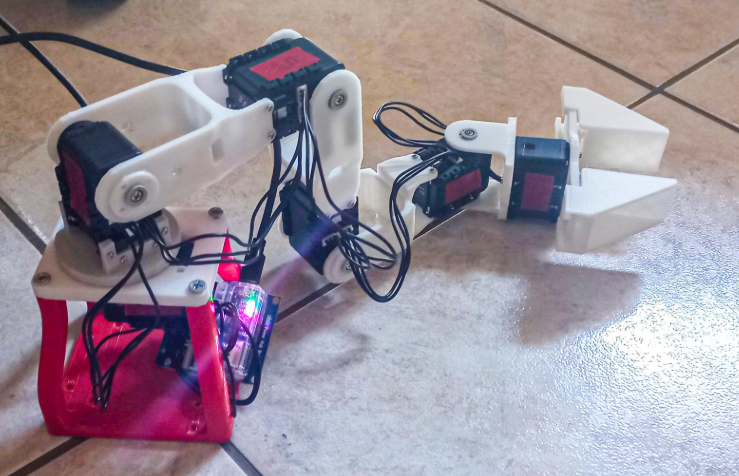
\includegraphics[width=0.90\textwidth]{reacher_robot.png}
    \caption{Visual representation of the Reacher robotic arm in the simulation environment.}
    \label{fig:reacher_robot}
\end{figure}

\subsection{Dataset Specifications}
For each robot, the available datasets containing synchronized logs of the robot’s state and movements were used for training and evaluation. The problem is formulated as learning the inverse kinematics function $dq = f(x, q, dx)$.
The dimensionality of the input and output spaces varies for each robot configuration, as summarized in following table.

\begin{table}[h]
    \centering
    \label{tab:datasets}
    \begin{tabular}{lcccc}
        \toprule
        \textbf{Robot} & \textbf{Task Space ($x$)} & \textbf{Joint Space ($q$)} & \textbf{Input Dim ($X$)} & \textbf{Output Dim ($Y$)} \\
        \midrule
        Reacher3 & $\mathbb{R}^{2}$ & $\mathbb{R}^{3}$ & 7 & 3 \\
        Reacher4 & $\mathbb{R}^{3}$ & $\mathbb{R}^{4}$ & 10 & 4 \\
        Reacher6 & $\mathbb{R}^{3}$ & $\mathbb{R}^{6}$ & 12 & 6 \\
        \bottomrule
    \end{tabular}
    \caption{Summary of dataset dimensions and spaces.}
    \end{table}

\subsection{Dataset Versions}
Two versions of the datasets were provided (Version 1 and Version 2). These versions likely differ in the random seed used for data generation, providing a way to test the robustness of the model.
In this report is primarily focused on \textbf{Version 1} for training and hyper-parameter tuning. However, the proposed pipeline is generic and can be applied to Version 2 without modifications.

\section{Baseline Evaluation: Linear Regression}

Given that the objective is to predict continuous joint displacements ($dq$) based on the robot's current state and target, the problem is naturally formulated as a regression task. 
Before exploring more expressive deep learning architectures, a baseline was established using a standard \textbf{Linear Regression} model. Although such a model was expected to be inadequate for capturing the nonlinear trigonometric relationships inherent in robotic kinematics, this step served two essential purposes:
\begin{enumerate}
    \item Verify the integrity of the data preprocessing pipeline.
    \item Empirically quantify the non-linearity of the problem.
\end{enumerate}

The model was trained on the standardized training set (80\% of the dataset) of the \textit{Reacher3} robot and evaluated on the held-out test set (20\%). 
The predefined random split (using \texttt{random\_state=42}) was strictly maintained to ensure that the evaluation was performed on unseen data and to allow fair comparison with subsequent neural network models.

\begin{figure}[h!]
    \centering
    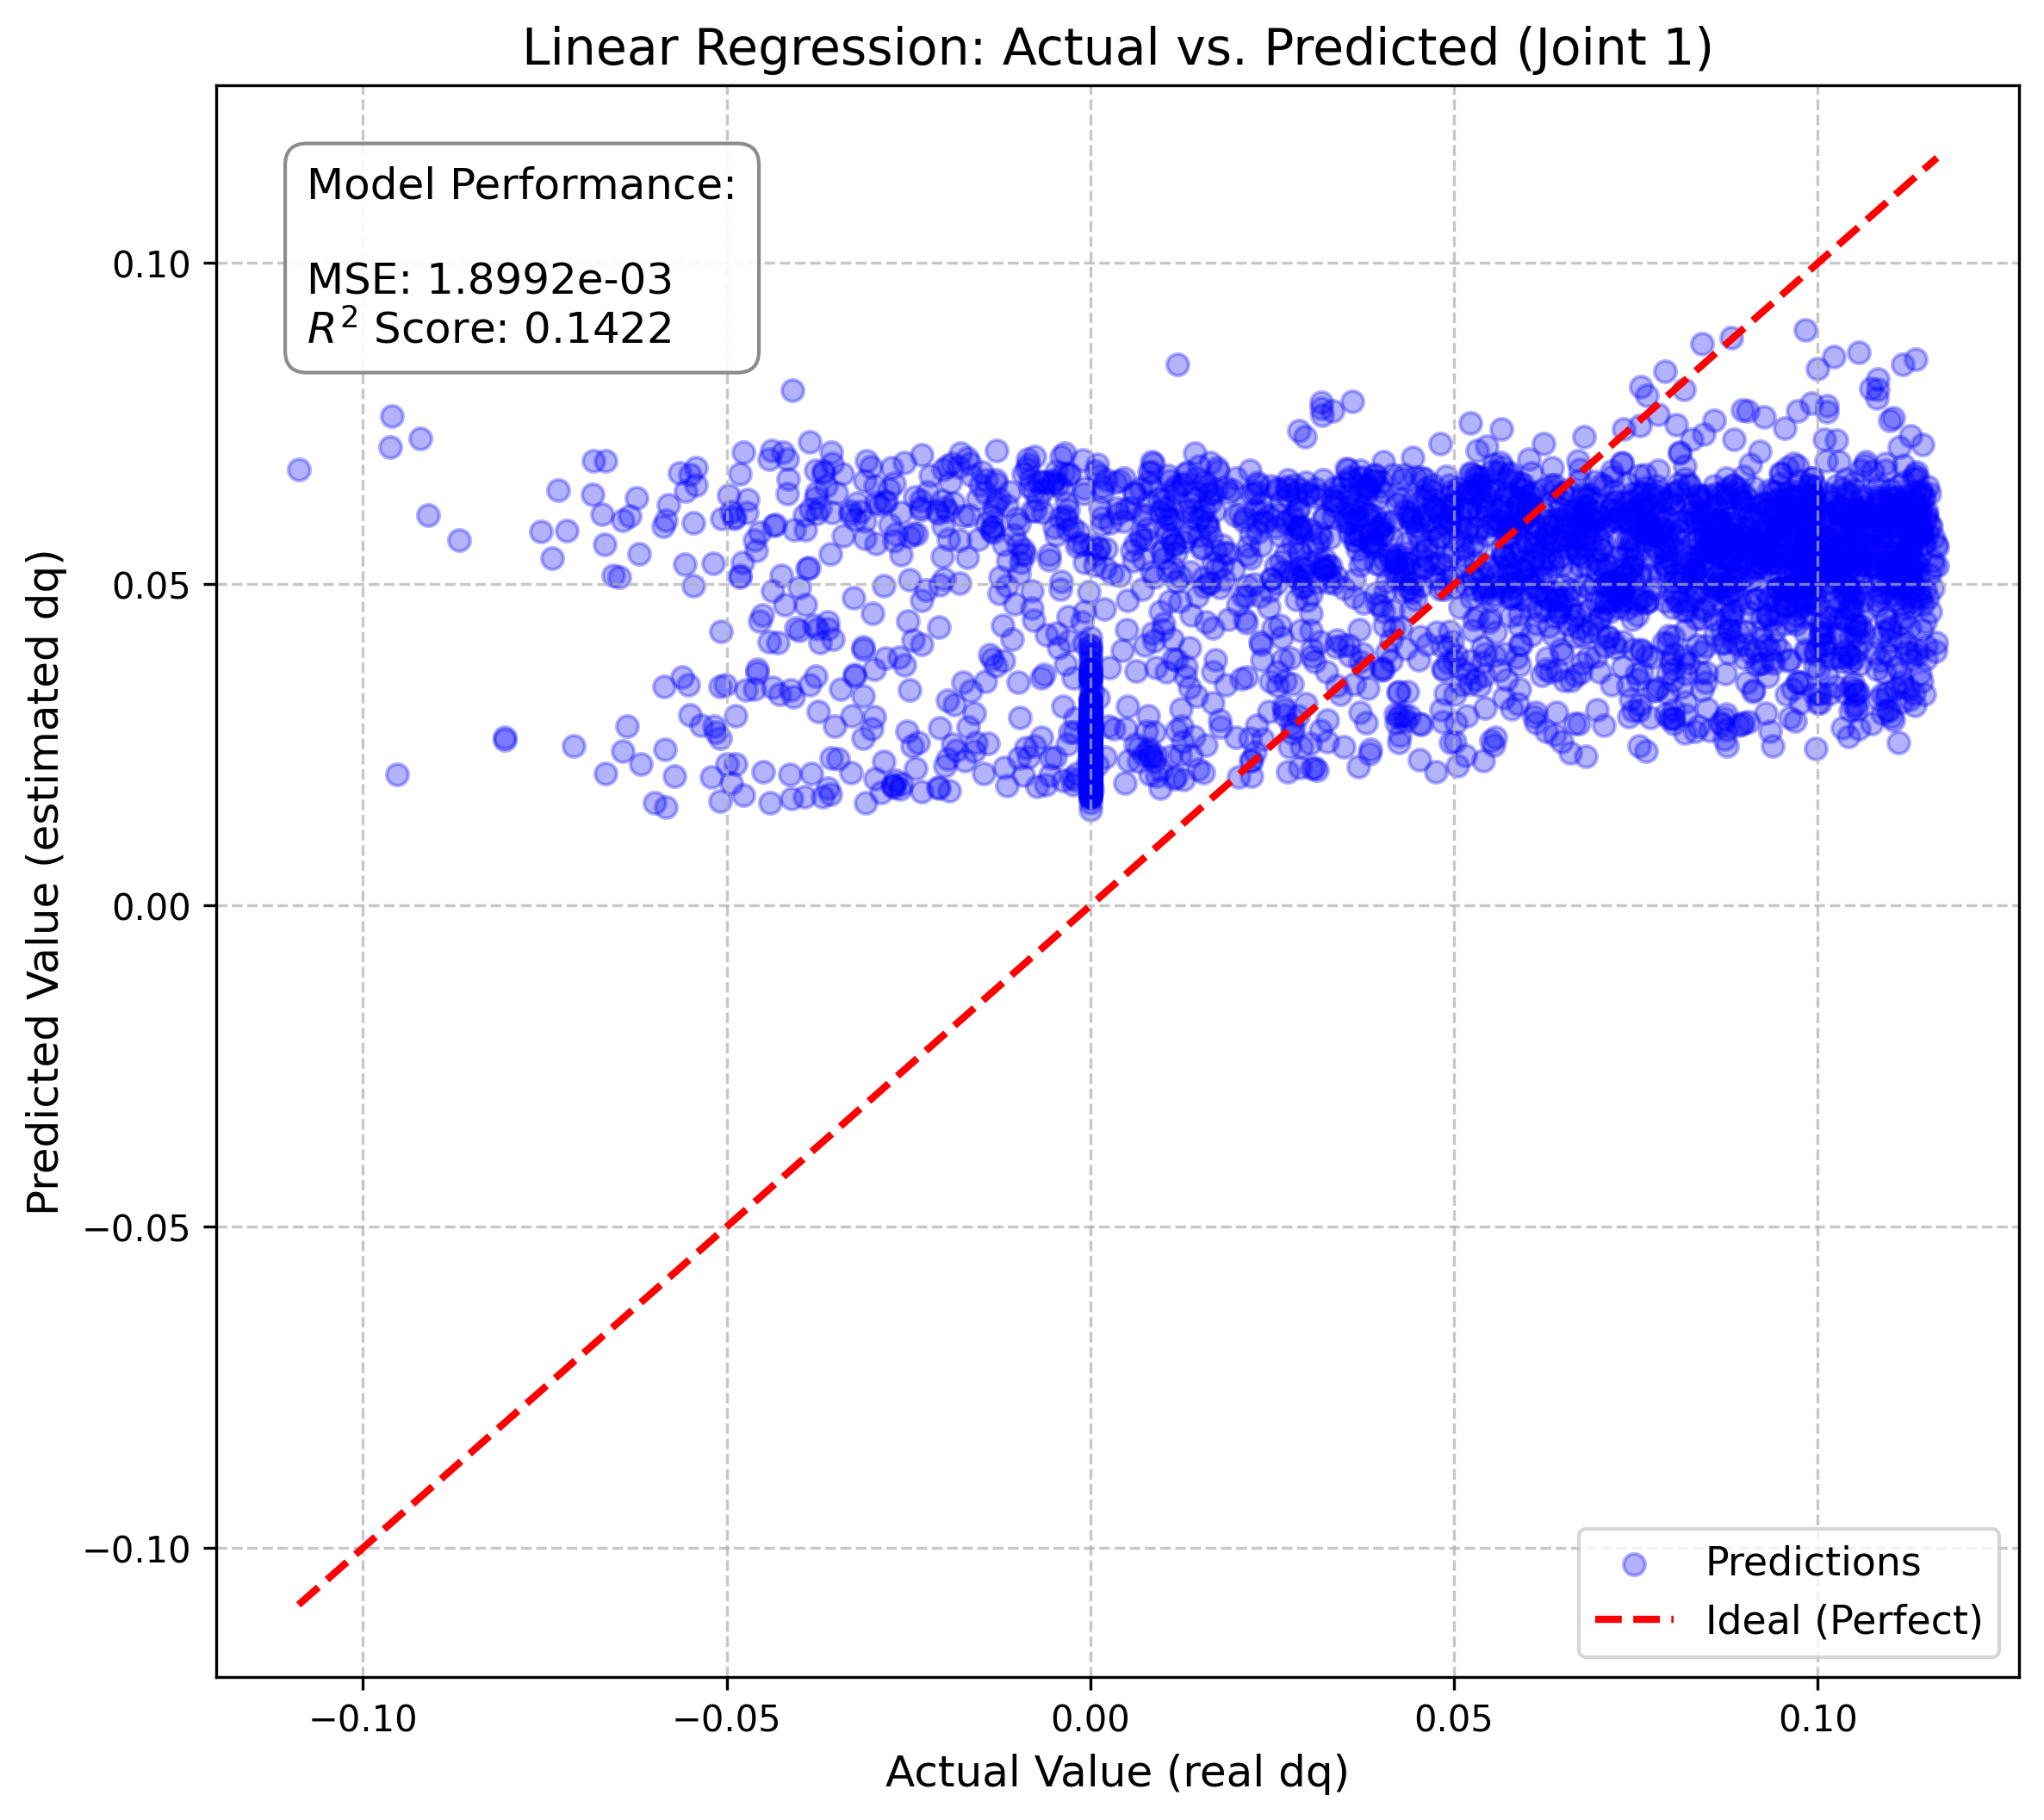
\includegraphics[width=0.85\textwidth]{linear_regression_results_eng.png}
    \caption{Visual evaluation of the Linear Baseline.}
    \label{fig:linear_baseline}
\end{figure}

The results, visualized in Figure \ref{fig:linear_baseline}, confirm the limitations of a linear approach. The model achieved an $R^2$ score of only \textbf{0.1422} and a Mean Squared Error (MSE) of approx. $1.9 \times 10^{-3}$. 
As shown in the scatter plot, the predictions (blue dots) fail to follow the ideal diagonal line (red dashed line) and instead form a dispersed cloud. This visually demonstrates that the relationship between the inputs ($x, q, dx$) and the output ($dq$) is highly non-linear, justifying the need for a more capable estimator such as a Feed-Forward Neural Network.

\section{First Approach: Feed-Forward Neural Network (MLP)}

Following the limited performance of the linear baseline, a non‑linear estimator based on a \textbf{Multi-Layer Perceptron (MLP)}.  The model was developed using the \texttt{TensorFlow} and \texttt{Keras} frameworks.
This section describes the architectural design, the motivation behind the chosen activation functions and optimizers, and the adopted training strategy.

\subsection{Model Architecture}
The network architecture was defined using the \texttt{Sequential} API. A fully connected (Dense) structure was selected, as it represents the standard choice for tabular regression problems in which spatial correlations (as in CNNs) or temporal dependencies (as in RNNs) are not explicitly present in the input features.

The specific configuration is as follows:
\begin{itemize}
    \item \textbf{Input Layer:} Implicitly defined with a shape of $(7,)$, corresponding to the input features: current position $x \in \mathbb{R}^2$, joint configuration $q \in \mathbb{R}^3$, and target displacement $dx \in \mathbb{R}^2$.
    
    \begin{figure}[H]
        \centering
        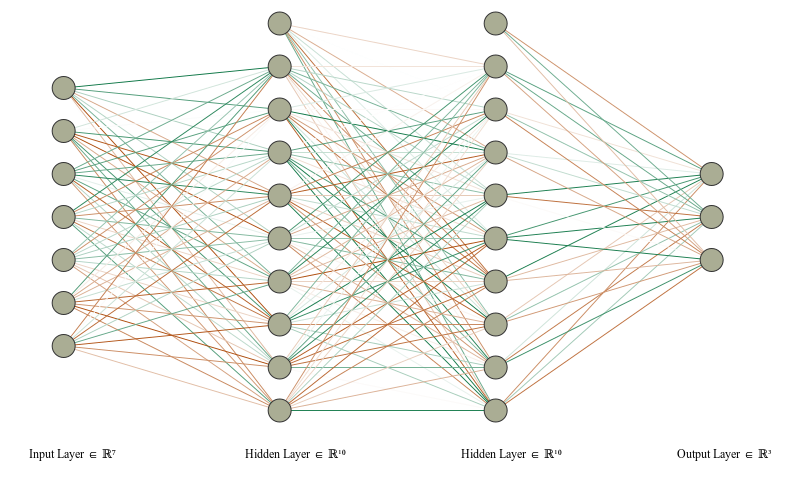
\includegraphics[width=0.90\textwidth]{nn_architecture.png}
        \caption{Architecture of the Feed-Forward Neural Network used for the Reacher3 robot.}
        \label{fig:nn_architecture}
    \end{figure}

    \item \textbf{Hidden Layers:}Two hidden layers were employed, each composed of 64 neurons.
    This depth allows the network to learn hierarchical representations of the kinematic function. The first layer captures simple correlations between joint angles and position, while the second layer combines these features to approximate the non-linear manifold of the robot's workspace.
    
    \item \textbf{Output Layer:} A dense layer with 3 neurons, corresponding to the required joint displacements $dq = (\delta q_1, \delta q_2, \delta q_3)$.
\end{itemize}

\subsubsection{Hidden Activation: ReLU}
For the hidden layers, are selected the \textbf{Rectified Linear Unit (ReLU)} as the activation function. 
We chose ReLU over traditional sigmoid or tanh functions for several reasons:
\begin{enumerate}
    \item \textbf{Sparsity:} ReLU outputs true zero for negative inputs, leading to sparse representations which are computationally efficient.
    \item \textbf{Gradient Propagation:} Unlike sigmoid/tanh, ReLU does not saturate for positive values. This mitigates the "vanishing gradient" problem, allowing deeper networks to learn faster and more effectively during backpropagation.
    \item \textbf{Non-linearity:} Despite being piecewise linear, ReLU introduces the necessary non-linearity to approximate complex functions, such as the inverse kinematics of a robotic arm.
\end{enumerate}

\subsubsection{Output Activation: Linear}
A \textbf{linear} activation function (identity mapping) was used for the final output layer:
\begin{equation}
    f(x) = x
\end{equation}
This is a critical choice for regression tasks. Unlike classification (where outputs are probabilities between 0 and 1) or bounded problems, the robot's joint displacements ($dq$) can be positive, negative, or zero, and represent physical quantities in radians. A linear activation ensures the output is unbounded, allowing the network to predict the exact magnitude and direction of the movement.

\subsection{Loss Function and Optimization}
To train the model, an objective function and a weight‑update algorithm were required.

\paragraph{Loss Function: Mean Squared Error (MSE)}
The \textbf{Mean Squared Error (MSE)} loss was adopted, as it penalizes larger prediction errors more strongly than smaller ones, making it suitable for continuous regression tasks.

\paragraph{Optimizer: Adam}
Model parameters were updated using the \textbf{Adam} optimizer. Although Stochastic Gradient Descent (SGD) represents a common alternative, Adam was preferred due to its robustness on non-linear regression problems and its ability to adapt learning rates during training—an advantage for the highly non-linear inverse‑kinematics mapping considered in this work.

\begin{itemize}
    \item \textbf{Handling Non-Stationary Objectives:} The loss landscape of kinematic functions involves complex trigonometric transformations and is highly non-convex. Adam's ability to maintain per-parameter learning rates allows it to navigate this complex surface more effectively than SGD, reducing the risk of getting stuck in local minima or saddle points.
    \item \textbf{Faster Convergence:} Given the iterative nature of our experiments, training speed was a priority. Adam utilizes momentum  to accelerate descent in relevant directions and dampen oscillations, leading to faster convergence with fewer epochs.
    \item \textbf{Robustness to Hyperparameters:} Adam performs well with default parameters (learning rate $\alpha \approx 10^{-3}$ or $10^{-4}$), which allowed us to focus our hyperparameter tuning efforts on the network architecture rather than spending excessive time manually tuning learning rate decay schedules required by SGD.
\end{itemize}

\subsection{Training Strategy}
The training process was configured with the following parameters:
\begin{itemize}
    \item \textbf{Epochs:} 50. An epoch represents one complete pass of the entire training dataset through the neural network. 50 epochs were deemed a reasonable starting point to observe convergence without excessive computational cost.
    \item \textbf{Batch Size:} 32. This defines the number of samples processed before the internal model parameters are updated. A size of 32 provides a good balance between the stability of the gradient estimate and training speed.
    \item \textbf{Validation Split:} 20\%. A portion of the training data was reserved to validate the model at the end of each epoch. This allows monitoring for overfitting (where training loss decreases but validation loss increases).
\end{itemize}

\subsection{Initial Results}
The model was trained on the standardized dataset for Reacher3. Upon completion, the model was saved in the HDF5 format (`.h5`) for future inference steps.

\begin{figure}[H]
    \centering
    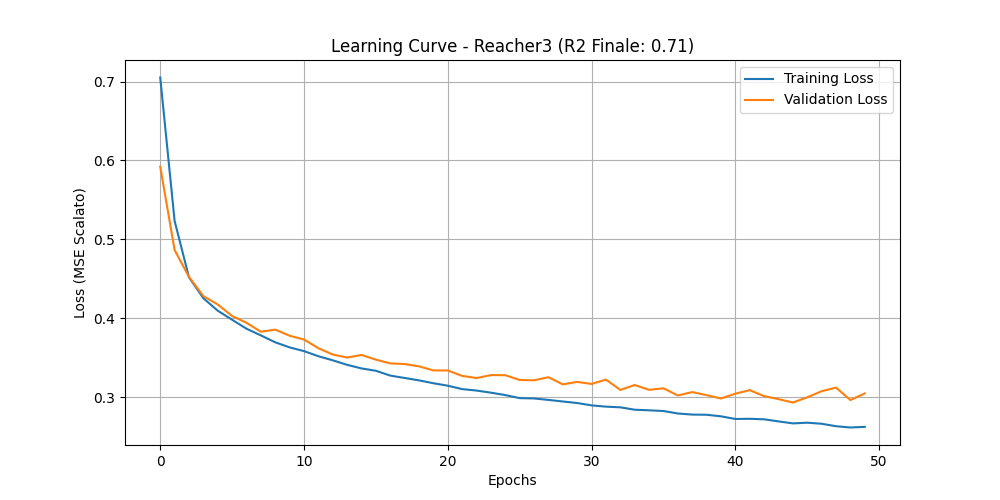
\includegraphics[width=0.95\textwidth]{learning_curve_reacher3.png}
    \caption{Learning curve of the first MLP model. Both training and validation loss decrease steadily, indicating successful learning without immediate overfitting.}
    \label{fig:learning_curve_initial}
\end{figure}

As shown in Figure \ref{fig:learning_curve_initial}, the loss decreases rapidly in the first 10 epochs and stabilizes around epoch 40.
The evaluation on the held-out Test Set yielded an \textbf{$R^2$ score of approximately 0.71}. 
While this is a significant improvement over the linear baseline ($0.14$), it suggests that the model captures the general trend of the motion but still lacks the precision required for fine-grained control, motivating further optimization (Hyper-parameter search).

\section{Evolution of the Approach}

The initial MLP model provided a decent baseline ($R^2 \approx 0.71$), but demonstrated that simply stacking layers was not sufficient to reach high precision. To improve performance, a systematic optimization process was followed, involving hyper-parameter tuning, feature engineering, and comparative analysis.

\subsection*{Hyper-parameter Search (Grid Search)}
It was hypothesized that the network capacity might be insufficient. To test this, a systematic grid search was performed, varying two key parameters:

\begin{itemize}
    \item \textbf{Network Width:} Comparing 64 vs. 128 neurons per layer.
    \item \textbf{Training Duration:} Comparing 50 vs. 100 epochs.
\end{itemize}

The search revealed that increasing model complexity (128 neurons) and training time (100 epochs) improved performance up to $R^2 \approx 0.75$. However, further increasing the size led to diminishing returns, suggesting that the bottleneck was not just network capacity, but the data representation itself.

\subsection*{Feature Engineering: Handling Angular Discontinuities}
A critical analysis of the dataset revealed a potential issue for regression models: the \textbf{angular discontinuity}. Joint angles are periodic (e.g., $-\pi$ and $\pi$ are the same physical position), but numerically far apart.
To address this, explicit \textbf{feature engineering} was introduced: instead of using the raw angle $q_i$, the input vector was augmented with the pair $(\sin(q_i), \cos(q_i))$.
\[
\text{Input}_{new} = [x, \sin(q), \cos(q), dx]
\]
This transformation removed singularities and provided a continuous representation of the kinematic chain.
\textbf{Result:} This single change boosted the performance on Reacher3 to \textbf{$R^2 \approx 0.78$}, confirming that injecting domain knowledge (trigonometry) is more effective than "brute-force" learning.

\subsection*{Comparative Analysis: XGBoost vs. Neural Networks}
To verify if the problem could be solved by simpler algorithms, the MLP was benchmarked against XGBoost.
The ensemble model achieved a significantly lower score ($R^2 \approx 0.65$) compared to the neural network. As visualized in Figure \ref{fig:xgboost}, the decision tree ensemble approximates the function via discrete splits (step-functions), leading to a high variance in predictions. This result confirms that the kinematic function $f(x,q,dx)$ is smooth and continuous---a domain where Neural Networks (universal function approximators) inherently outperform partition-based algorithms.

\begin{figure}[H]
    \centering
    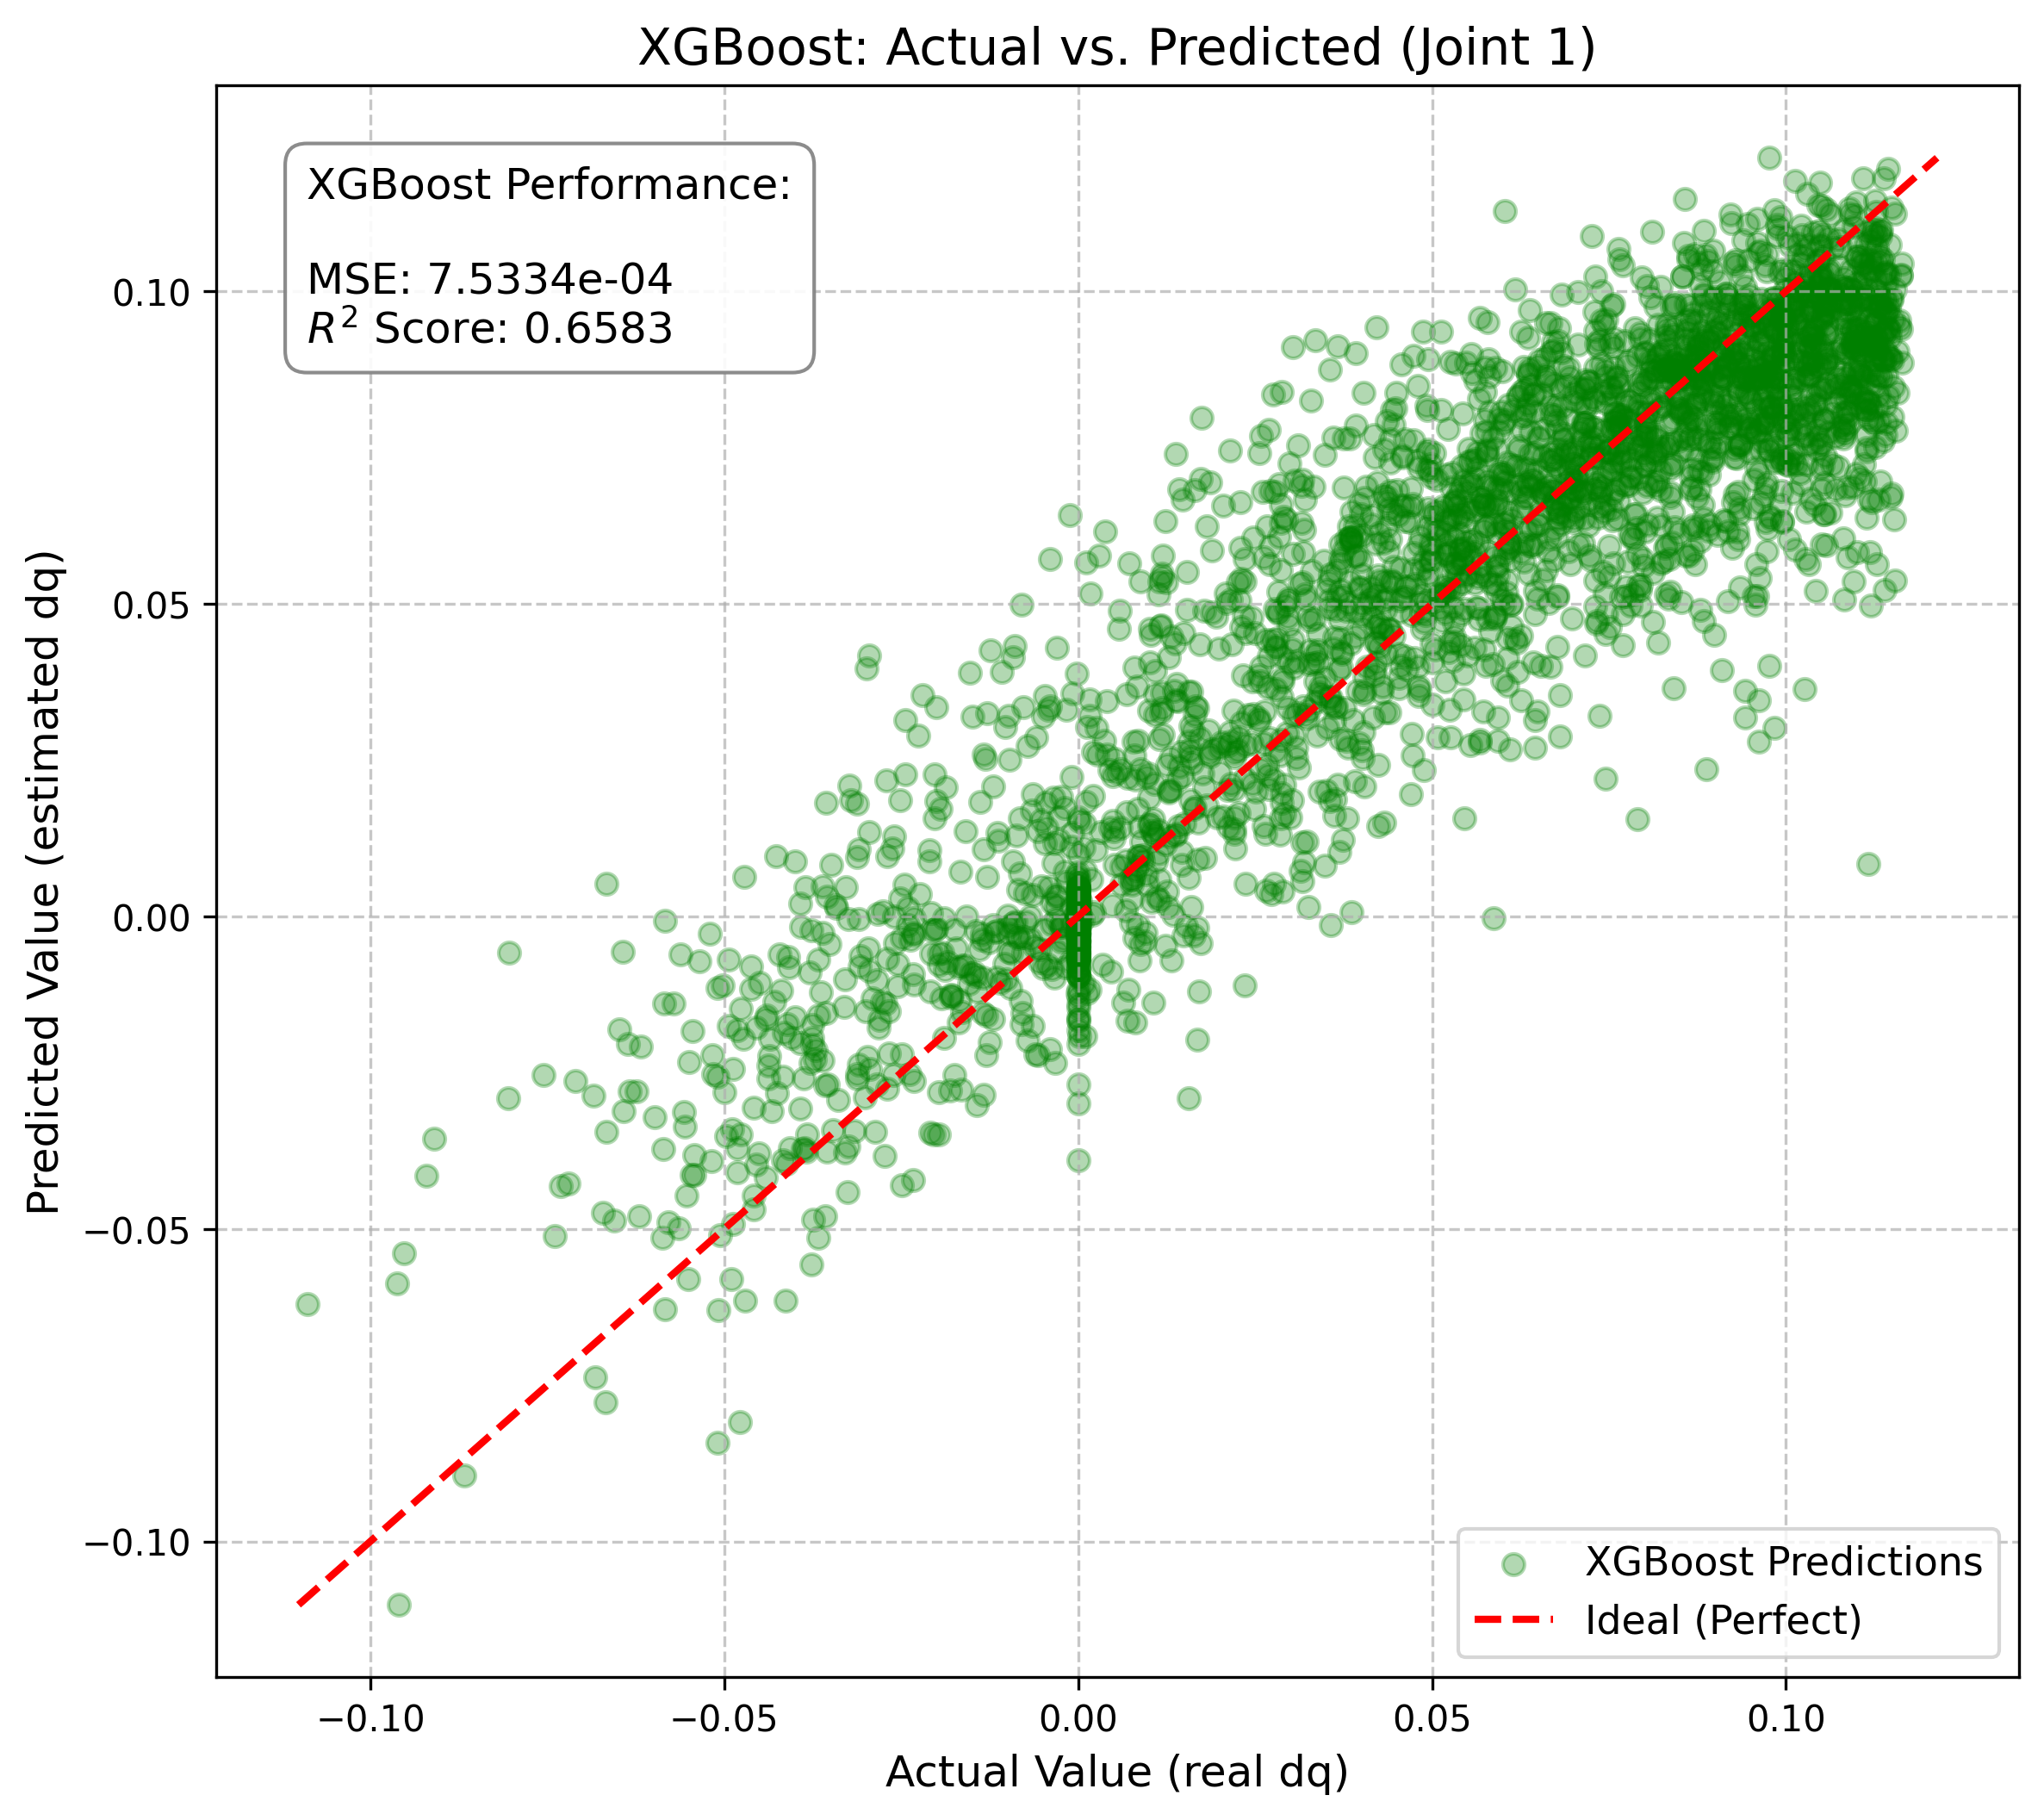
\includegraphics[width=0.7\textwidth]{xgboost_results.png}
    \caption{XGBoost predictions. The dispersed points illustrate the difficulty of modeling continuous kinematic smoothness with discrete decision trees.}
    \label{fig:xgboost}
\end{figure}

The scatter plot reveals that while XGBoost approximates the general trend better than linear regression ($R^2=0.52$ vs $0.14$), it still struggles to perfectly align along the diagonal (the ideal behavior). The visible dispersion of points indicates that the discrete decision boundaries of the tree ensemble fail to capture the fine-grained smoothness of the robotic function $f(x, q, dx)$.

\section{Final Solution: Automated Experimental Framework}
As the complexity of the experiments increased (varying architectures, dropout rates, and robot types), manual management of training runs became error-prone. To address this, was developed a robust, interactive software framework designed to ensure \textbf{reproducibility} and \textbf{scalability}.

The pipeline was engineered with three core capabilities:
\begin{itemize}
    \item \textbf{Dynamic Configuration:} Architecture (depth, width) and regularization parameters (Dropout) are injected at runtime, facilitating rapid A/B testing.
    \item \textbf{Structured Artifact Serialization:} For every experiment, the system automatically serializes the trained model weights (`.h5`), the specific feature scalers (`.pkl`), and training logs. This ensures that any result presented in this report can be precisely reproduced.
    \item \textbf{Standardized Evaluation:} All models are evaluated on a held-out test set using identical metrics, ensuring fair comparability between simple (Reacher3) and redundant (Reacher6) robots.
\end{itemize}

\section{Architectural Optimization on Reacher3}
\label{sec:reacher3_optim}

To determine the optimal network capacity before scaling to redundant robots, was conducted a controlled ablation study on the Reacher3 planar arm (Dataset Version 1). This robot served as an ideal testbed due to its lower computational overhead, allowing for rapid iteration.

It was evaluated three distinct configurations, varying network width (neurons per layer) and depth against training duration. All experiments utilized the automated framework described in Section 6, with Dropout enabled to strictly assess generalization capability.

\subsection{Results and Cost-Benefit Analysis}
Table \ref{tab:reacher3_experiments} summarizes the performance metrics. The primary objective was to maximize the $R^2$ score on the test set while minimizing training latency.

\begin{table}[h]
    \centering
    \label{tab:reacher3_experiments}
    \begin{tabular}{lcccc}
        \toprule
        \textbf{Architecture} & \textbf{Epochs} & \textbf{Training Time} & \textbf{Test $R^{2}$} & \textbf{$\Delta R^2$ vs Baseline} \\
        \midrule
        \textbf{[256, 256, 128]} & \textbf{300} & \textbf{1m 52s} & \textbf{0.7929} & \textbf{--} \\
        {[}512, 512, 128{]} & 300 & 3m 03s & 0.7962 & +0.0033 \\
        {[}512, 512, 256{]} & 400 & 2m 15s & 0.7940 & +0.0011 \\
        \bottomrule
    \end{tabular}
    \caption{Ablation study on Reacher3. Increasing complexity yields diminishing returns.}
\end{table}

\subsection{Discussion}
The empirical data reveals a clear phenomenon of \textbf{diminishing returns}:

\begin{itemize}
    \item \textbf{Inefficiency of Large Models:} Doubling the hidden layer width (from 256 to 512 neurons) increased the training time by approximately 63\% (from 1m 52s to 3m 03s) but yielded a negligible accuracy improvement of only $0.0033$ in $R^2$.
    \item \textbf{Depth vs. Smoothness:} Adding a deeper third layer (increasing the final layer from 128 to 256 units) did not improve performance ($0.7940$ vs $0.7962$). This confirms that the inverse kinematics of the planar arm is a relatively smooth function that does not require the highly complex decision boundaries typical of deeper architectures.
    \item \textbf{Selection of the Baseline:} Based on these findings, we selected the \textbf{[256, 256, 128]} configuration as the optimal trade-off between computational cost and predictive accuracy.
\end{itemize}


\section{Comprehensive Results Analysis}

Across all experiments performed on the three robots (Reacher3, Reacher4 and Reacher6), using both Dataset Version 1 and Version 2, was observed consistent trends. For comparability, Table~\ref{tab:best_results_all} reports the best configuration obtained on Dataset Version 1 for each robot, which provides stable behavior and similar difficulty across settings.

\begin{table}[h!]
    \centering
    \label{tab:final_summary}
    \begin{tabular}{lccc}
        \toprule
        \textbf{Architecture} & \textbf{Epochs} & \textbf{Time} & \textbf{Test $R^{2}$} \\
        \midrule
        \textbf{[256, 256, 128]} & \textbf{300} & \textbf{1m 52s} & \textbf{0.7929} \\
        {[}512, 512, 128{]} & 300 & 3m 03s & 0.7962 \\
        {[}512, 512, 256{]} & 400 & 2m 15s & 0.7940 \\
        \bottomrule
    \end{tabular}
    \caption{Best-performing configurations for each robot on Dataset Version 1.}
    
\end{table}

A first observation is the clear relationship between robot complexity and achievable accuracy: Reacher3 (3 DoF) reaches almost $R^2 = 0.79$, Reacher4 (4 DoF) drops to approximately $0.71$, and Reacher6 (6 DoF) stabilizes around $R^2 = 0.45$. 
This reflects the increasing redundancy and nonlinearity of the inverse-kinematics mapping as the number of joints increases.

All models were trained with dropout enabled, which helped stabilize training and reduce overfitting, particularly for Reacher4 and Reacher6.

\subsection{Learning Curves Analysis}

To better understand these differences, Figures~\ref{fig:curve_reacher3}--\ref{fig:curve_reacher6} report the learning curves of the best model for each robot, together with a brief interpretation of their distinctive behaviors.

\subsection*{Reacher3}
    \begin{figure}[H]
    \centering
    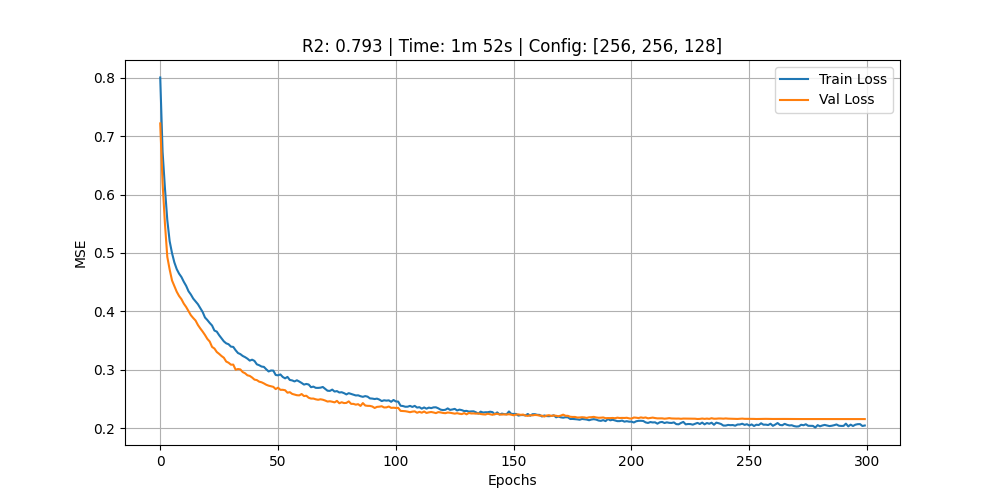
\includegraphics[width=0.95\textwidth]{reach3_256_125_128_300.png}
    \caption{Learning curve for Reacher3}
    \label{fig:curve_reacher3}
    \end{figure}

    Figure~\ref{fig:curve_reacher3} shows the training and validation loss curves for the best-performing model on Reacher3,
    highlighting several desirable properties:

    \begin{itemize}

    \item \textbf{Fast initial convergence.}  
    Both training and validation loss drop sharply in the first $\sim$20 epochs, 
    indicating that the network quickly learns the dominant structure of the 
    inverse-kinematics mapping.

    \item \textbf{Stable mid- to late-training phase.}  
    Between 50 and 300 epochs, the loss decreases gradually and consistently, 
    without oscillations or sudden spikes.

    \item \textbf{Minimal overfitting.}  
    The validation loss closely tracks the training loss throughout the entire 
    training process.  
    This indicates that the network capacity is well matched to the complexity 
    of the task and that the use of dropout effectively prevents the model from 
    overfitting.

    \item \textbf{Near-zero generalization gap.}  
    The gap between training and validation loss is very small, especially in the
    final 100 epochs.  

    \item \textbf{Efficient training time (1m 52s).}  
    Despite the 300 epochs, training is fast thanks to the small input dimension 
    and the relatively compact architecture.

\end{itemize}


\subsection*{Reacher4}

    \begin{figure}[H]
    \centering
    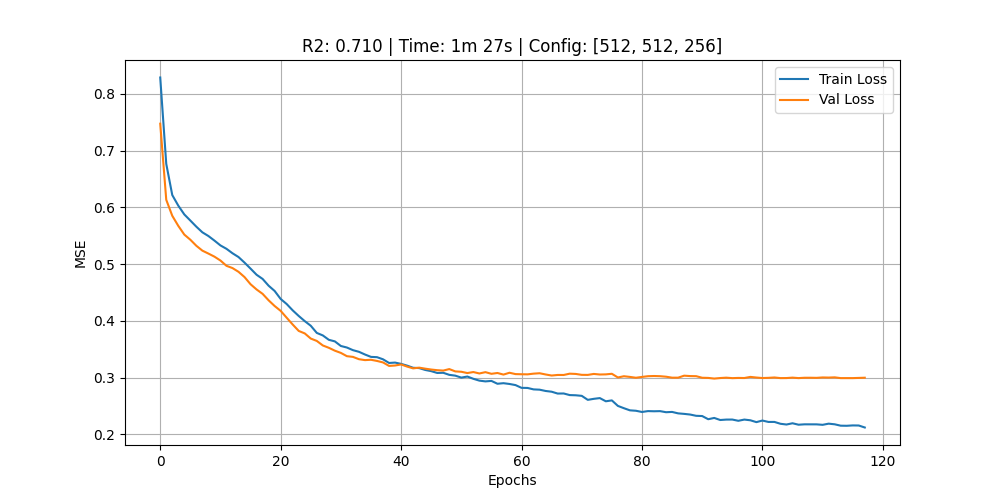
\includegraphics[width=0.95\textwidth]{reach4_512_512_256.png}
    \caption{Learning curve for configuration Reacher4.}
    \label{fig:curve_reacher4}
    \end{figure}

    Compared to Reacher3, the behavior of the learning curve reveals several key 
    differences tied to the increased dimensionality of the robot (4 DoF instead of 3):

\begin{itemize}

    \item \textbf{Slower convergence in the initial phase.}  
    The loss decrease in the first 20--30 epochs is less steep than in Reacher3.
    This suggests that the network requires more time to learn the higher-dimensional 
    nonlinear relationships of a 4-DoF kinematic chain.

    \item \textbf{Early plateau in validation loss.}  
    Starting at approximately epoch 50, the validation loss flattens and shows
    limited improvement for the remaining epochs.  
    This indicates that the model reaches its generalization capacity relatively 
    early, while additional training mostly improves the training loss.

    \item \textbf{Clear generalization gap.}  
    Unlike Reacher3, where training and validation curves almost overlap, 
    Reacher4 displays a noticeable gap:  
    training loss continues to decrease steadily, while validation loss stabilizes.  
    This suggests that the kinematic function for Reacher4 is more complex and 
    that the current model architecture—although large—may still be underfitting 
    in some regions of the input space.

    \item \textbf{Surprisingly fast training time (1m 27s).}  
    Despite using a larger architecture (\texttt{512–512–256}), Reacher4 trains 
    faster than both Reacher3 and Reacher6.  
    This confirms the earlier observation that \textbf{epoch count is not a 
    reliable predictor of training time}: the data dimensionality and batch 
    characteristics have a stronger impact on computational cost.

\end{itemize}

\subsection*{Reacher6}

    \begin{figure}[H]
    \centering
    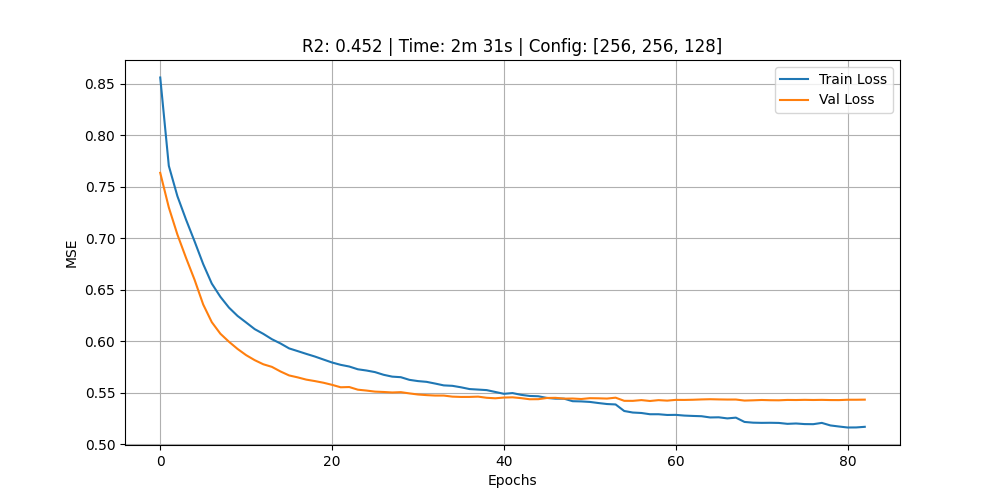
\includegraphics[width=0.95\textwidth]{Reach6_256_256_128_500.png}
    \caption{Learning curve for Reacher6.}
    \label{fig:reacher3_512_256}
    \end{figure}
     \noindent

    Among the three robots considered, Reacher6 presents the most challenging 
    learning landscape. With 6 degrees of freedom and a high-dimensional joint 
    space, the mapping from $(x, q, dx)$ to $dq$ becomes considerably more complex 
    and highly redundant. This complexity is clearly reflected in the learning 
    curve:

\begin{itemize}

    \item \textbf{Fast initial drop but slower convergence than Reacher3/4.}  
    Within the first 20 epochs, both training and validation loss decrease 
    sharply, showing that the model quickly captures some global structure.  
    However, after this initial phase, improvements become much slower than in 
    Reacher3 or Reacher4.

    \item \textbf{Pronounced generalization gap.}  
    The validation loss stabilizes around epoch 30--40, while the training loss 
    continues to decrease for the entire duration of training.  
    This gap indicates that the model is fitting the training set more than the 
    validation set, but still does not have enough capacity to fully capture the 
    functional complexity required for accurate predictions.

    \item \textbf{Validation loss saturates early.}  
    Unlike Reacher3, where validation loss continues to improve for nearly 250 
    epochs, in Reacher6 the validation curve becomes almost flat after 40 epochs.  
    This suggests that the dataset may not provide sufficient information for the 
    model to learn a more accurate mapping, or that a deeper/wider architecture 
    is required.

    \item \textbf{High training time (2m 31s).}  
    Using the same \texttt{[256, 256, 128]} architecture as Reacher3, training 
    takes considerably longer.  
    This is caused by the increased input dimensionality and higher computational 
    cost of processing 6-DoF data, confirming that \textbf{time per epoch is not 
    comparable across robots}.

    \item \textbf{Limited maximum accuracy ($R^2 \approx 0.45$).}  
    Even with 500 epochs, the model reaches a significantly lower performance 
    than for Reacher3 and Reacher4.  
    This is expected: inverse kinematics for a 6-DoF manipulator is highly 
    redundant, many-to-one, and requires more expressive function approximators.

\end{itemize}

\subsection{Summary}

Overall, these results show that:
\begin{itemize}
    \item MLPs model low-dimensional robots effectively (Reacher3).
    \item Increasing robot redundancy reduces achievable accuracy (Reacher4).
    \item High-dimensional robots require deeper or more expressive models 
          (Reacher6).
\end{itemize}

Despite differences in convergence behavior, dropout consistently helped stabilize 
training for all models.

\section{Conclusion}
In this project, robotic control was addressed as a supervised learning task to approximate the inverse kinematics function $dq = f(x, q, dx)$ without prior knowledge of the robot's geometric model.
The experimental analysis followed an evolutionary path that highlighted three key findings:

\begin{enumerate}
    \item \textbf{Validation of Non-Linearity:} The failure of the linear baseline ($R^2 \approx 0.14$) empirically confirmed that the trigonometric transformations intrinsic to robotic motion require universal non-linear approximators.
    
    \item \textbf{The Role of Domain Knowledge:} It was demonstrated that "brute-force" capacity scaling is less effective than targeted feature engineering. The introduction of explicit $(\sin(q), \cos(q))$ transformations to handle angular discontinuities was the decisive factor in stabilizing learning.
    
    \item \textbf{The Redundancy Barrier:} The comparison across morphologies revealed a clear performance boundary. While the MLP approach excels in deterministic systems (Reacher3, $R^2 \approx 0.79$), it degrades significantly on highly redundant manipulators (Reacher6, $R^2 \approx 0.45$). This occurs because the static network, lacking temporal context, attempts to average out the infinite valid joint configurations for a single end-effector position.
\end{enumerate}

\section*{Acknowledgment of Generative AI Usage}
In compliance with the assignment guidelines, I declare the use of Google Gemini for coding assistance (debugging TensorFlow pipelines) and LaTeX formatting. All experimental results and analysis are my own work.

\end{document}
